For the purposes of writing this thesis, an implementation of the grammatical evolution algorithm was developed using the object-oriented paradigm in the C++ language. This system can be used to generate and evolve programs in any arbitrary language, used to solve any arbitrary problem.

The classes written for this generic part of the implementation are:

\begin{list}{$\bullet$}{}  	
	\item \textbf{GrammaticalEvolution} - the top class in the hierarchy, used to encapsulate the process of mapping a unit's genotype onto its phenotype
	\item \textbf{Grammar} - the class used for reading and parsing the .bnf files, and also storing information about a grammar and its productions 
	\item \textbf{Crossover} - an implementation of the crossover operator
	\item \textbf{Mutation} - an implementation of the mutation operator
	\item \textbf{Unit} - the class used for storing information about a unit
	\item \textbf{Node} - the process of the genotype-phenotype mapping is implemented using linked lists, and this class encapsulates nodes in this list
	\item \textbf{Symbol} - a class used in the genotype-phenotype mapping, stores information about the contents of each node in the linked list
	\item \textbf{GrammarParsingState} - the process of reading and parsing the .bnf file is implemented as a final automata, and this enumeration stores all the states of that automata
	\item \textbf{SymbolType} - an enumeration which stores all types which an instance of the class Symbol can have, and the types are terminal and nonterminal
	\item \textbf{DecodeException} - a class used for handling all potential problems during the process of parsing a .bnf file
\end{list}

The other part of the implementation is the classes used for the purpose of evolving cache replacement policies. These classes are:

\begin{list}{$\bullet$}{}  	
	\item \textbf{Strategy} - the base class for a cache replacement strategy
	\item \textbf{GEStrategy} - the class used for the strategies generated by the GrammaticalEvolution
	\item \textbf{GeneratedStrategies} - the class which stores all generated strategies in one place; this class has to be recompiled during each iteration of the genetic algorithm
	\item \textbf{FIFO} - an implementation of the FIFO strategy
	\item \textbf{LRU} - an implementation of the LRU strategy
	\item \textbf{LFU} - an implementation of the LFU strategy
	\item \textbf{CLOCK} - an implementation of the CLOCK strategy
	\item \textbf{OPT} - an implementation of the OPT strategy
\end{list}

For the sake of simplicity and the adherence to the 'separation of concerns' principle, the main function was split into six files, each with its own main function. These files are:

\begin{list}{$\bullet$}{}  	
	\item \textbf{init} - initializes a random population and stores each unit's genotype in a separate file inside the /solutions directory
	\item \textbf{decode} - reads the genotypes of every unit inside the current population and decodes their genotypes onto their phenotypes, which are then stored inside the GeneratedStrategies
	\item \textbf{run} - tests all strategies from the GeneratedStrategies using the train data, and stores their scores inside the /results directory
	\item \textbf{evolution} - reads each strategy's score and performs the evolutionary process of creating a new generation, which is then stored inside the /solutions directory
	\item \textbf{test\_generated\_strategy} - simulates a generated strategy using the test data and outputs its hit count
	\item \textbf{test\_heuristic\_strategies} - simulates the heuristic strategies using the test data and outputs their hit counts
\end{list}

During each iteration of the evolutionary process, new strategies are generated and stored as C++ files, which need to be compiled before they can be run. The class responsible for decoding the genotype of each unit, which is an array of 8-bit numbers, to its corresponding phenotype, which is a computer program, is the GrammaticalEvolution class. This class has a $decode$ method which takes as input some Unit and returns its phenotype representation as a string. This string needs to be properly placed into a specific file, so that it can be correctly compiled and run. This is the responsibility of the main loop of the program. This main loop isn't written as a C++ file, instead it is a bash script. This bash script manages and calls the six files which do a specific part of the evolutionary process, recompiles the parts of the code that change during each iteration, and assures the persistency of the generated strategies between each run. Each strategy has a genotype, phenotype and score, and each of these is stored inside a different textual file.

Figure A.1 shows a class diagram of the complete project. The classes which belong to the core part of the project and which can be applied to any problem are colored in blue. The classes which are specifically built for the problem of evolving cache replacement strategies are colored in green. These classes are shown without their member variables and functions since these are unimportant in viewing the whole project and the connections between its parts. Finally, the six C++ files which are being compiled to executable programs and subsequently run by the main bash script are colored in yellow. These aren't classes so they technically don't belong in a class diagram, but they were included for the sake of showing all the built components and their connections. The diagram was built using the tool \citep{diagrams}.

\begin{figure}[H]
	\centering
	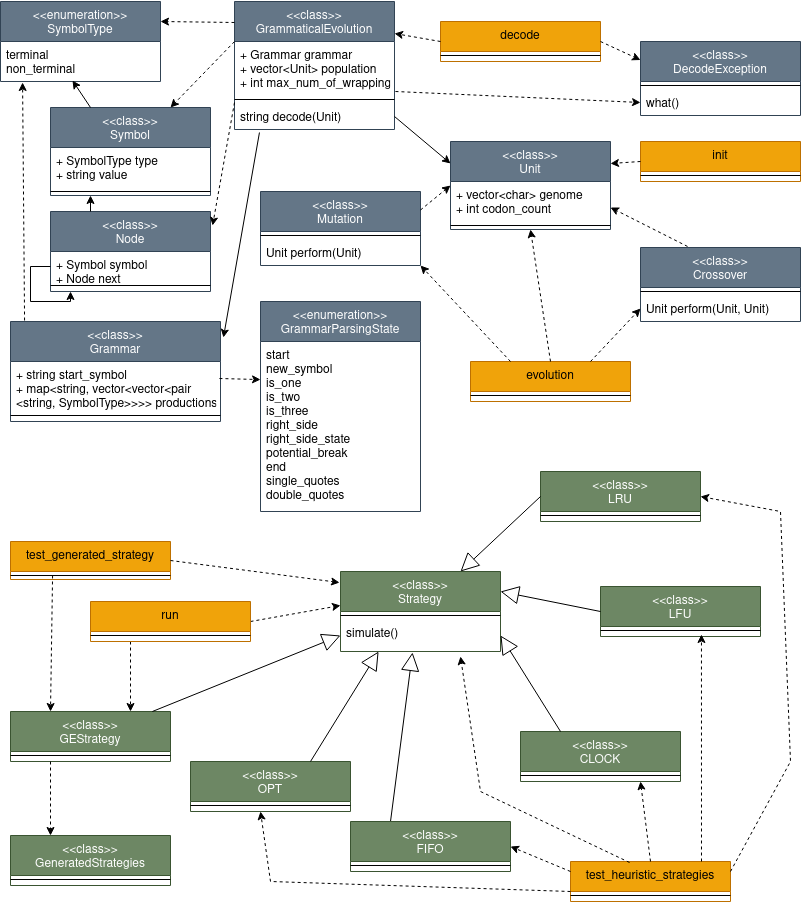
\includegraphics[scale=0.55]{class_diagram.png}
	\caption{Class diagram}
\end{figure}